
In this thesis, all the simulations are based on the geometry of a skew quadrupole which belongs to the group of high-order corrector magnets designed for the High-Luminosity LHC upgrade. The skew quadrupole is developed by the LASA laboratory of INFN-Milano. Its geometry is presented in Fig. \ref{fig:Skew_quad_geometry}. Each coil of the skew quadrupole (marked in red in the left picture) is fully impregnated and positioned in two mechanical supports (marked in grey). The entire magnet is surrounded by an iron yoke (marked in blue). One coil of a magnet out of four in total is presented in the right picture.

\begin{figure}[H]
    \centering
    \begin{tikzpicture}
    \node at (0,0) {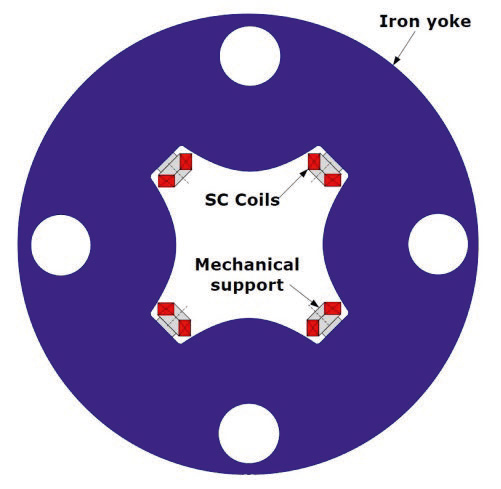
\includegraphics[width=0.3\linewidth]{sections/1D_quench_modelling/figures/geometry/Quadrupole_Cross_Section.png}};
    \node at (5,0) {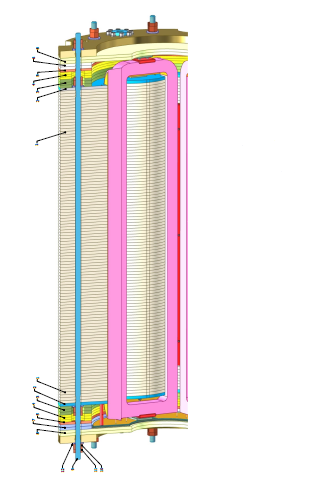
\includegraphics[width=0.225\linewidth]{sections/1D_quench_modelling/figures/geometry/SkewQuad3D.png}};
    \end{tikzpicture}
     \caption{Left: cross-section of the skew quadrupole~\cite[p.~103-105]{hl_lhc_tech_design_report_v01}; right: one coil of the skew quadrupole~\cite{marco_prioli_mails}.}
    \label{fig:Skew_quad_geometry}
\end{figure}

As presented in Fig.~\ref{fig: 1d_strand_geometry}, the coil consists of a composite strand marked in yellow made of Nb-Ti and a copper stabiliser. The strand is fully insulated with an S2-glass material marked in red. The cable is wound 754 times to form a coil with the total length of 812~m~\cite{samuele_mariotto_mails}. After the winding process, the coil is impregnated with an epoxy resin CTD-101K marked in blue in Fig.~\ref{fig: 1d_strand_geometry}. The Rutherford cable is not applied in high-order corrector magnets. In the remainder of the thesis, the term "cable" is restricted to the composite strand made of a superconductor and a copper stabiliser including an external insulation layer and, optionally, a resin filler. The bare cable and winding are referred to as "strand". The one-dimensional coordinate system $\bar x$ in Fig.~\ref{fig: 1d_strand_geometry} represents the longitudinal direction of the strand. The 1D geometry is based on geometrical parameters of a single strand of the skew quadrupole whose simulations are further described in the next section. 

\begin{figure}[H]
    \centering
    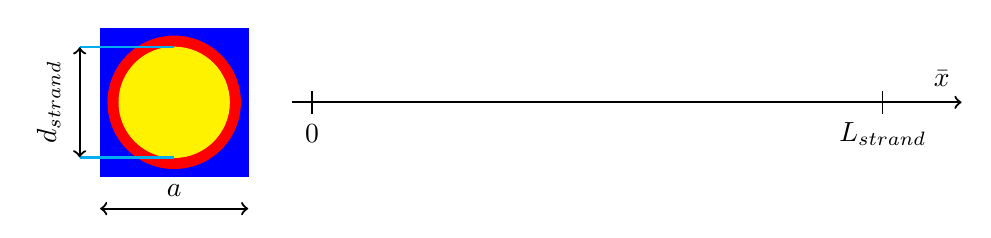
\begin{tikzpicture}[scale = 1]
        \filldraw[blue] (-0.941,-0.941) rectangle (0.941,0.941);
        \filldraw[red] (0,0) circle (0.7+0.07*2);
        \filldraw[yellow] (0,0) circle (0.7);
        \draw[thick, cyan] (-0.8*1.5,0.7) -- (0,0.7);
        \draw[thick, cyan] (-0.8*1.5,-0.7) -- (0,-0.7);
        \draw[black, thick, <->] (-0.75*1.6,0.7) -- (-0.75*1.6,-0.7);
        \node[scale = 1, rotate=90] at (-1.1*1.45, 0) {$d_\text{strand}$};
        \draw[thick,<->] (-0.941,-0.9*1.5) -- (0.941,-0.9*1.5);
        \node[scale = 1] at (0, -0.7*1.6) {$a$};
        \draw[thick,->] (1.5,0) -- (10.0,0);
        \draw[thin] (1.75,-0.15) -- (1.75,0.15);
        \draw[thin] (9,-0.15) -- (9,0.15);
        
        \node[scale = 1] at (9.75, 0.3) {$\bar x$};
        \node[scale = 1] at (9, -0.4) {$L_\text{strand}$};
        \node[scale = 1] at (1.75, -0.4) {0};
        
    \end{tikzpicture}
    \caption{1D strand geometry.}
    \label{fig: 1d_strand_geometry}
\end{figure}

The parameters of the skew quadrupole presented in Table \ref{table:skew_quad_params_table_basic} do not change in the remainder of the thesis. The last two: $(i)$ residual resistivity ratio, RRR, $(ii)$ copper-to-superconductor ratio, $r_\text{Cu/sc}$ are obtained from the measurements of the prototype magnet performed at INFN.~\cite{marco_prioli_mails}

\begin{table}[H]
    \caption{Geometrical parameters of the skew quadrupole \cite{hl_lhc_tech_design_report_v01, marco_prioli_mails}.} 
    \vspace{-1.em} 
    \fontsize{10}{10}
    \selectfont 
    \renewcommand{\arraystretch}{1.5}
    \begin{center}
    \begin{tabular}{ ccc }  
    \hline
    parameter & value & unit \\
    \hline
    $d_\text{strand}$ & 0.7 & [mm] \\
    $a$ & 0.941 & [mm] \\
    $r_\text{Cu/sc}$ & 2.2 & [-] \\
    RRR & 193 & [-] \\  
    \hline 
    \end{tabular}
    \end{center}  
     \label{table:skew_quad_params_table_basic} 
 \end{table}
